% ===================================================================
%                   Presentación con Latex Beamer
% ===================================================================
\documentclass[9pt,xcolor=svgnames]{beamer}
%\documentclass[handout,xcolor=svgnames]{beamer} %Version imprimible
% -------------------------------------------------------------------
% Paquetes personalizados
\usepackage{../paquetes}
\usepackage{../colores}
\usepackage{../info}
\usepackage{../modo}
% -------------------------------------------------------------------

% Comienza el documento
\begin{document}
% Tikz -> Imágenes
\tikzstyle{every picture}+=[remember picture]
% Entorno matemático
\everymath{\displaystyle}
% -------------------------------------------------------------------

% -------------------------------------------------------------------
% Fondo blanco: primera página
% ------------------------------------------------------------------

\beamersetaveragebackground{white}

\begin{frame}
 \thispagestyle{empty}
 
 \animate<2-3> 
 \begin{figure}[t]
  \centering
  \includegraphics<1>[scale=0.7]{../Imagenes/logo_1.pdf}
  \includegraphics<2>[scale=0.7]{../Imagenes/logo_2.pdf}
  \includegraphics<3>[scale=0.7]{../Imagenes/logo_3.pdf}
  \includegraphics<4>[scale=0.7]{../Imagenes/logo_4.pdf}
 \end{figure}
\end{frame}


% -------------------------------------------------------------------
% Fondo para el resto del documento
\setbeamertemplate{background}{

\includegraphics[width=\paperwidth,height=\paperheight]
{../Imagenes/fondo.pdf}
}
% -------------------------------------------------------------------


% Continuación:
% Transparencia de Inicio -> Título
\begin{frame}
 \titlepage
\end{frame}

\normalsize

% Transparencia de índice
\begin{frame}{Índice} 
 \transboxin
 \tableofcontents
\end{frame}
  
  
 \section{Estado del proyecto}
 
  \subsection{Actualización de la planificación}
  
  \begin{frame}{Diagrama de Gannt}
   \transdissolve
   
   \begin{figure}[t]
    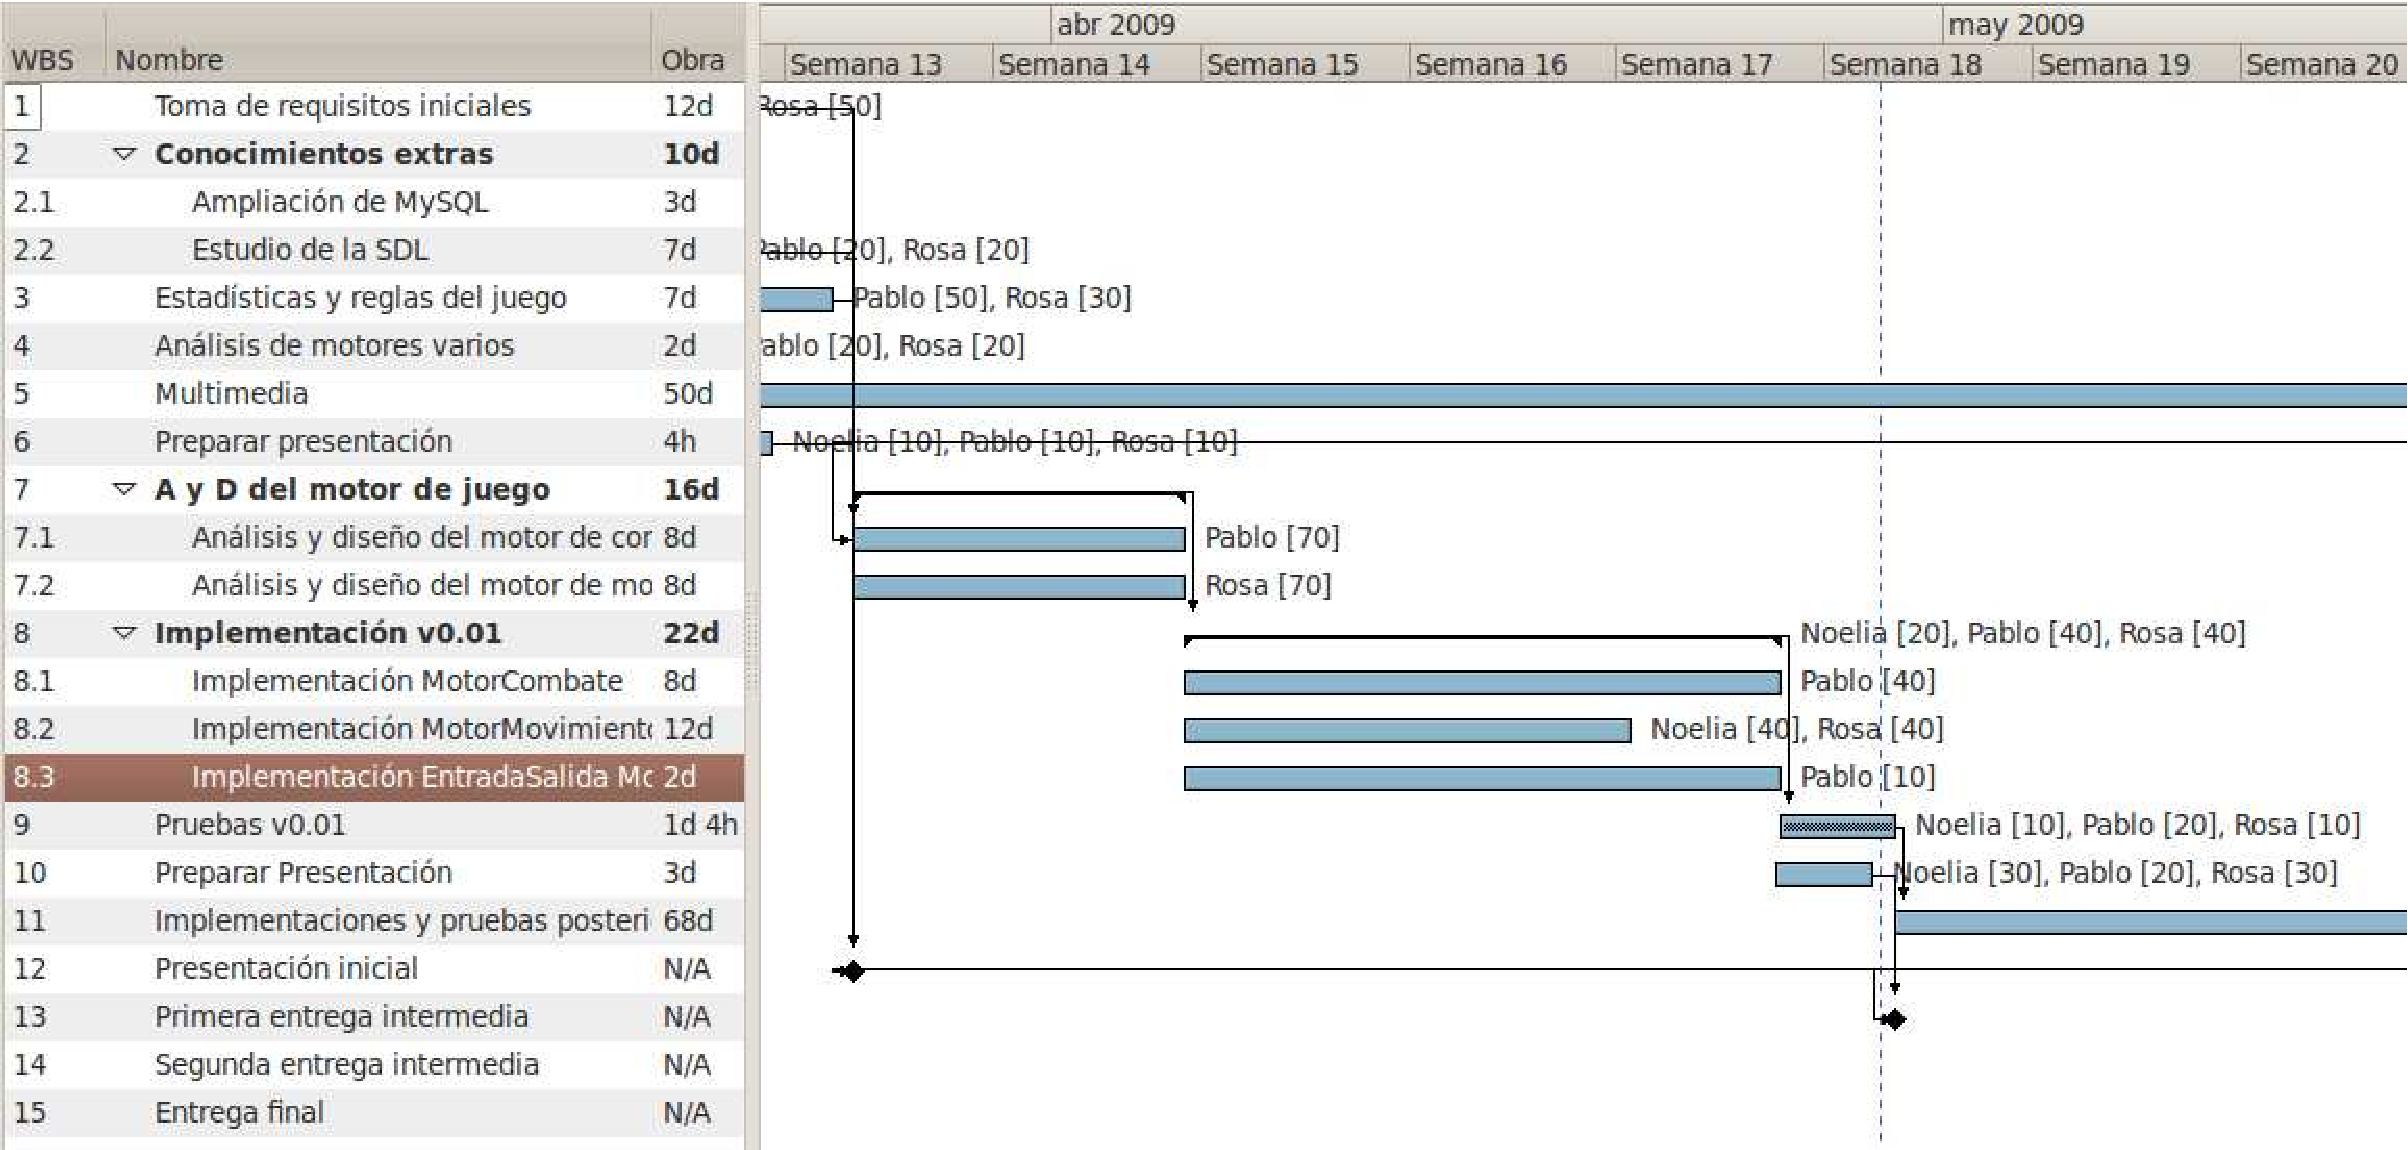
\includegraphics[scale=0.27]{./Imagenes/gannt.pdf}
   \end{figure}
   
  \end{frame}
  
  
  \begin{frame}{Asignación de Recursos}
   
   Actualmente centrándonos en la implementación:
   
   \begin{block}{Motor de combate}
    \begin{itemize}
     \item Desarrollador principal: Pablo.
     \item Estado actual: versión de prueba de combate sin gráficos.
     \item A completar: parte gráfica.
    \end{itemize}
   \end{block}

   \begin{block}{Motor de movimiento}
    \begin{itemize}
     \item Desarrolladoras principales: Rosa y Noelia.
     \item Estado actual: finalizados los elementos necesarios para el 
	   movimiento básico y la visualización de gráficos, así como los de 
	   gestion de eventos externos. 
     \item A completar: sección correspondiente a los menús y a la
	   carga/guardado de niveles.
    \end{itemize}
   \end{block}
    
  \end{frame}
   
   
   
   \subsection{Modificaciones sufridas por el proyecto}
   
   \begin{frame}{Modificaciones y justificaciones}
    
    \begin{block}{Utilización de ficheros XML}
     Para guardar la configuración del juego, así como para ``diseñar'' y
     mantener en un formato simple la distribución de los diferentes
     niveles de juego.\\
     
     Potenciamos así la posibilidad de que se incrementen los niveles del
     juego.
    \end{block}
    
   \end{frame}
   
   
   
 \section{Calidad del proyecto software}
 
  \subsection{Ingeniería del software}
  
  \begin{frame}{Modelo incremental aplicado al proyecto}   
   \transdissolve
   
   Basándonos en nuestra experiencia, está resultando bastante apropiado.
   
   \begin{itemize}
    \item Modificar conforme se observan posibles mejoras.
    \item No abarcar demasiado para una versión primitiva. Poco a poco.
   \end{itemize}
   
  \end{frame}
  
  \subsection{Ejemplo: Análisis y diseño del motor gráfico}
  
  \begin{frame}{Diagrama de Casos de Uso}

   \begin{figure}[t]
    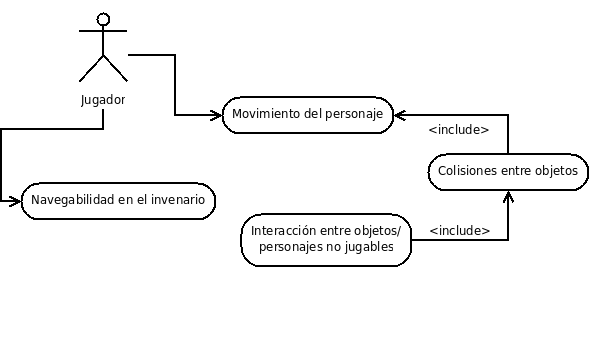
\includegraphics[scale=0.4]{./Imagenes/Diagrama_Casos_Uso.png}
   \end{figure}
  \end{frame}
  
  
  
  \begin{frame}{Ejemplo: Descripción Caso de Uso}
   
   Movimiento del personaje.
   
   \begin{itemize}
    \item \textbf{Caso de Uso:} Movimiento del personaje.
    \item \textbf{Descripción:} El jugador podrá realizar cuatro tipos de
	  movimientos con el personaje principal: trasladar el personaje
	  hacia arriba, hacia abajo, hacia la derecha o hacia la
	  izquierda del mapa.
    \item \textbf{Actores:} Usuario o jugador del videojuego.
    \item \textbf{Precondiciones:} El videojuego está iniciado y está
	  cargado todo el motor de movimiento sin errores.
    \item \textbf{Postcondiciones:} Ninguna.
    \item \textbf{Escenario principal:} \\
	  
	  \begin{enumerate}
	   \item El jugador pulsa la tecla 'up' del teclado.
	   \item El sistema mueve el personaje del juego hacia arriba
		 del mapa.
	   \item El jugador colisiona con un objeto. \textbf{Include:
		 Colisiones entre objetos.}
	  \end{enumerate}
   \end{itemize}
  \end{frame}
  
  
  \begin{frame}{Ejemplo: Descripción Caso de Uso}
   \begin{itemize}
    
    \item \textbf{Escenarios alternativos o de error:} \\
	  \begin{itemize}
	   \item \textbf{1a} El jugador pulsa la tecla 'down' del teclado.
	   \item \textbf{  } El sistema mueve el personaje del juego
		 hacia abajo del mapa.
	   \item \textbf{1b} El jugador pulsa la tecla 'left' del teclado.
	   \item \textbf{  } El sistema mueve el personaje del juego
		 hacia la izquierda del mapa.
	   \item \textbf{1c} El jugador pulsa la tecla 'right' del teclado.
	   \item \textbf{  } El sistema mueve el personaje del juego
		 hacia la derecha del mapa.
	   \item \textbf{1d} El personaje se encuentra en un borde de la
		 pantalla y quiere avanzar (cualquier dirección).
	   \item \textbf{ 1} El sistema comprueba que existe más mapa
		 fuera de la pantalla y hace que el personaje acceda a
		 esa porción del mapa.
	   \item \textbf{ 2} El sistema comprueba que no existe más mapa
		 para visualizar en dicha dirección y deja al personaje
		 en la misma posición.
	  \end{itemize}
   \end{itemize}
   
   
  \end{frame}
  
  
  
  \begin{frame}{Diagrama de Casos de Uso}
   \begin{figure}[t]
    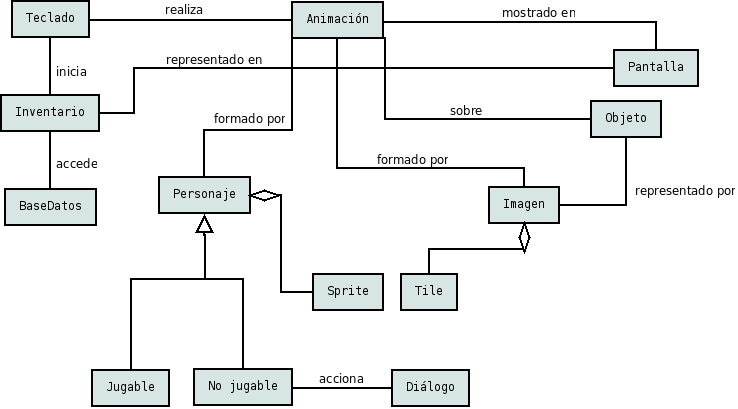
\includegraphics[scale=0.34]{./Imagenes/Diagrama_conceptual.png}
   \end{figure}
  \end{frame}
  
  
  
 \section{Resultados obtenidos}
 
  \subsection{Algoritmo general en pseudocódigo}

  \begin{frame}{Algoritmo}
   
   \noindent Se ejecuta el programa. \\
   Se cargan los ficheros de configuración. \\
   Se inicia el videojuego mostrando el menú principal.
   
   \begin{itemize}
    \item El jugador elige jugar.\\
	  Se muestra en pantalla las opciones de crear nuevo juego o
	  cargar uno existente.
	   
	  \begin{itemize}
	   \item El jugador crea un nuevo juego. \\
		 Se cargan los ficheros iniciales. \\
		 Se muestra
		 una animación de la introducción del juego.
		 
	   \item El jugador elige  cargar un juego existente. \\
		 Se cargan los ficheros configurados
		 para el usuario.
	  \end{itemize}
   \end{itemize}
   
  \end{frame}

  \begin{frame}{Algoritmo}
    
   El usuario comienza a jugar (con el motor de movimiento).\\ 
   El jugador mueve el personaje.
   
   \begin{itemize}
    \item El personaje se mueve sin ningún inconveniente.
    \item El personaje no se puede mover (colisiona con un objeto).
    \item El personaje no se puede mover pero si interactuar:
	  
	  \begin{itemize}
	   \item Comienza un combate.		  
	   \item Interactúa con un objeto.
	   \item Dialoga con otro personaje.  
		 
	  \end{itemize}
	  
   \end{itemize}
  \end{frame}
  
  
  \begin{frame}{Algoritmo}
   El jugador entra en el inventario.
   
   \begin{itemize}
    \item Visualiza la pestaña contenedora del estado de los
	  personajes.
    \item Visualiza la pestaña contenedora de los objetos que tiene el
	  grupo.
    \item Visualiza la pestaña que contiene las opciónes Guardar y
	  Salir.
	  
	  \begin{itemize}
	   \item El usuario guarda el juego.\\
		 El sistema guarda el estado del juego.
	   \item El usuario sale del juego.\\
		 El sistema destruye la memoria dinámica utilizada y
		 sale del programa.		  
	  \end{itemize}
   \end{itemize}
    
   El jugador elige salir.\\
   El sistema sale del programa.
  \end{frame}
    
    
  \subsection{Implementación}
  
  \begin{frame}{Clases ya implementadas}
   
   \begin{block}{Motores}
    \begin{columns}
     
     \begin{column}{3cm}
      \begin{block}{De combate}
       Atributos\\
       Atributos-base\\
       Combatiente\\
       Especial\\
       Grupo\\
       Habilidad\\
       Inventario\\
       Objeto      
      \end{block}
     \end{column}
     
     \begin{column}{2cm}
      \begin{block}{Gráfico}
       Animacion\\
       Evento\\
       Imagen\\
       Pantalla\\
       Personaje\\
       Sprite\\
       Tile
      \end{block}
     \end{column}
     
    \end{columns}
   \end{block}
  \end{frame}
  
  \begin{frame}{Para muestra...}
   
   No vamos a enseñar el código puesto que sería entrar demasiado en
   materia.\\
   
   Resulta más efectivo, y más entretenido ver como funciona.
   
  \end{frame}
  
  
  \subsection{Multimedia}
  
  \begin{frame}{Imagenes}
   TILES (Fuente: Battle for Wesnoth (GPL) - modificados)
   
   OBJETOS (Fuente: Battle for Wesnoth)
   
   SPRITES BASICOS + MENU + BOTONES + CURSOR (FLECHA) (Fuente: Propios)
  \end{frame}
  
  \begin{frame}{Audio}
   BSO: 
   
   Sonidos: Fuente: Battle for Wesnoth
   
   + Creative Commons
  \end{frame}
  
  
 \section{Metodología de trabajo}
 
  \subsection{SVN y forja}
  
  \begin{frame}{Trabajando en grupo}
   Revisión: 100\\
   
   Listas de correo para actualizaciones/commits importantes
  \end{frame}
  
  
  
  \subsection{Aplicaciones extras}
  
  \begin{frame}{Aplicaciones y elementos extras}
   \begin{itemize}
    \item Doxygen
    \item Netbeans
   \end{itemize}
  \end{frame}
  

  \subsection{Adorno del proyecto}
  
  \begin{frame}{Elementos extras}
   \begin{itemize}
    \item Página web
    \item Documentación actualizada a diario
    \item Manual de usuario en desarrollo ya colgado
   \end{itemize}
  \end{frame}
  
\end{document}
 